\documentclass[10pt]{article}
\usepackage[a4paper,margin=24mm]{geometry}
\usepackage[T1]{fontenc}
\usepackage{lmodern,microtype,amsmath,amssymb,amsthm,booktabs,graphicx,xcolor,listings,caption}
\usepackage[colorlinks=true,linkcolor=blue!45!black,citecolor=blue!45!black,urlcolor=blue!45!black]{hyperref}
\usepackage[round,authoryear]{natbib}
\usepackage{fancyhdr}
\pagestyle{fancy}\fancyhf{}\fancyhead[L]{\small Gupta \quad StopRisk}\fancyhead[R]{\small Research manuscript}\fancyfoot[C]{\thepage}\setlength{\headheight}{14pt}
\setlength{\parskip}{2pt}\setlength{\parindent}{1em}\brokenpenalty=10000
\newtheorem{theorem}{Theorem}
\newtheorem{proposition}[theorem]{Proposition}
\newcommand{\Prb}{\mathbb P}
\graphicspath{{figures/}}
\captionsetup{font=small,labelfont=bf}
\lstset{basicstyle=\ttfamily\small,breaklines=true,frame=single,columns=fullflexible}
\title{\vspace{-8mm}\textbf{StopRisk: Finite-Evidence Envelopes for\\ Shutdown-Based AI Control}}
\author{Shivam Gupta\\Independent Researcher\\\texttt{shivam1720406@gmail.com}}
\date{17 October 2026}
\begin{document}\maketitle
\begin{abstract}
AI-control evaluations often estimate whether an attack is caught before an uncaught harmful outcome occurs. A point estimate does not quantify the evidence supporting that probability, particularly when decisive events are rare or an attacker can switch strategies. We present StopRisk, an executable specialization of exact binomial inference and robust dynamic programming for a fixed menu of stationary attack kernels with immediate effective shutdown. Factoring each kernel into a decisive-event probability and a conditional harm share gives closed-form Bellman confidence operators. A single finite-sample confidence event bounds optimal attack risk simultaneously at every deployment horizon and permits subsequent selection within the declared evaluation family. We derive a bounded-switch structure and a block evaluator for the upper envelope. In 240,000 synthetic evaluation datasets, both the factorized method and a separately calibrated hazard-box baseline exceed 99\% coverage; neither uniformly minimizes interval width. In one rare-event condition, 73.72\% of datasets with 1,000 observations per attack give zero plug-in risk despite a true 100-opportunity risk of 1.89\%. Secondary analysis reconstructs eight count tables from published monitoring aggregates and illustrates the remaining uncertainty. These are model-conditional bounds over tested attacks, not certificates against untested strategies or changing deployment conditions.
\end{abstract}
\noindent\textbf{Keywords:} AI control; competing risks; finite-sample inference; robust dynamic programming; evaluation evidence.

\section{Introduction}
When a monitored agent is potentially adversarial, safety depends on the order of two events: an uncaught harmful action and a catch that terminates further opportunities. Successful detection can therefore reduce subsequent exposure. The probability of harm over a deployment differs from both per-attempt attack success and the probability of any harm without shutdown. AI control explicitly studies deployment protocols under intentional subversion \citep{greenblatt,griffin}. Recent attack-selection work already distinguishes finite-deployment safety from the catch fraction among decisive outcomes \citep{gewang}.

The question here is narrower: \emph{given finite evaluation counts for a declared menu of attacks, what uncertainty remains about harm before shutdown when an attacker can switch among those attacks?} An evaluator needs this uncertainty to assess whether a reported safety number supports a specified decision. Repeated simulation from a small empirical library can estimate the library's plug-in risk accurately while leaving substantial uncertainty about its generating probabilities.

We develop an explicit evidence-to-risk pipeline (Figure~\ref{fig:pipeline}). For each tested attack, we factor the three-outcome distribution into the frequency of decisive events and the conditional share of those events that are harmful. Exact binomial intervals produce inexpensive robust Bellman updates. The statistical event is established once, in the space of kernels; the resulting bounds hold simultaneously for every horizon. Deployment-time switching among tested kernels is included in the optimization.

\begin{figure}[ht]\centering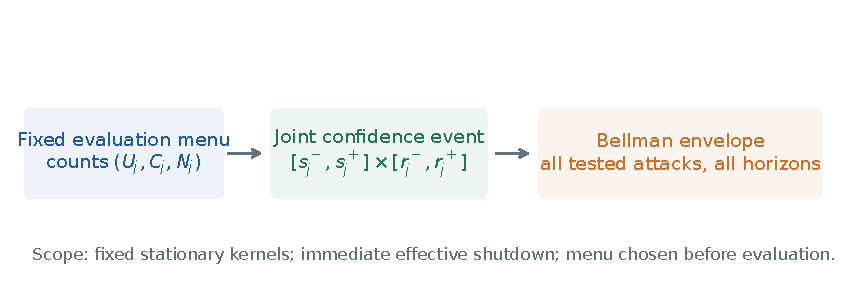
\includegraphics[width=\linewidth]{pipeline.pdf}
\caption{The proposed pipeline. The confidence event concerns fixed kernels estimated from evaluation data. Deployment-time selection occurs inside the Bellman calculation. Statistical coverage does not establish that the kernel model describes a real deployment.}\label{fig:pipeline}\end{figure}

Our contribution is an operational specialization with explicit assumptions, closed-form confidence operators, a bounded-switch computational characterization, and a reproducible study of informativeness. Its ingredients are established: exact binomial inference \citep{clopper}, robust dynamic programming \citep{iyengar,nilim}, and absorbing-state AI-control models \citep{griffin,gewang}. We do not claim to introduce these ingredients, strategic attack selection, or the fact that zero failures need not imply low risk. The proposed artifact combines them into a checkable calculation that handles empty decisive samples and selection across a finite evaluation family.

\section{Related work and contribution boundaries}
\paragraph{AI-control games and attack selection.}
\citet{greenblatt} evaluate protocols combining untrusted generation, monitoring, and limited auditing. \citet{griffin} formalize control evaluations as partially observable games, including finite horizons and resource-dependent behavior. \citet{gewang} demonstrate start and stop policies and derive the three-state finite-horizon safety expression used below. Their study discusses small effective sample sizes under selection. We extend neither the general game formalism nor their empirical attack-selection results; we study finite-evidence uncertainty in a restricted kernel model.

\paragraph{Competing outcomes and robust reachability.}
Harm and catch are competing absorbing outcomes. Cumulative-incidence inference has a substantial literature; \citet{blanche}, for example, develops profile-likelihood and constrained-bootstrap intervals. Our observations are complete categorical outcomes with constant probabilities per tested attack, permitting a simple conditional binomial factorization. The confidence limits are Clopper--Pearson limits \citep{clopper}. Their coverage is conservative, rather than equal to the requested level. Rectangular uncertainty and Bellman propagation are classical \citep{iyengar,nilim}. General piecewise-affine Bellman reachability is also studied in formal verification \citep{varonka}. Our scalar specialization admits an explicit switch bound and geometric block evaluation; it is not a new general-purpose robust-MDP algorithm.

\paragraph{Evaluation practice.}
ControlArena supplies safety metrics and percentile-bootstrap utilities \citep{controlarena}; its tutorial already warns about low sample sizes and uninformative perfect-safety estimates. We do not characterize those warnings as absent. The public factorial study \citep{williams} provides independent aggregate data for a secondary calculation. Our bootstrap baseline is a specifically defined conditional procedure, not a replication or an audit of ControlArena's bootstrap. A contemporaneous assurance essay studies finite-evidence limits in repeated red-team/blue-team matrix games \citep{tmls}; our estimand is absorbing-event risk under adaptive selection from stationary kernels.

\section{Model, estimand, and assumptions}\label{sec:model}
Fix a finite menu $\mathcal A=\{1,\ldots,K\}$. On each opportunity, before observing that opportunity's random outcome, the attacker selects $j\in\mathcal A$. Conditional on this selection and all past information, the outcome is
\begin{equation}
H\text{ with probability }u_j,\quad C\text{ with probability }c_j,\quad
N\text{ with probability }1-u_j-c_j.\label{eq:kernel}
\end{equation}
Here $H$ is uncaught harm, $C$ is a catch followed by effective shutdown, and $N$ is continuation. Both $H$ and $C$ absorb the process. Parameters satisfy $u_j,c_j\geq0$ and $u_j+c_j\leq1$. Define
\begin{equation}
s_j=u_j+c_j,\qquad r_j=u_j/(u_j+c_j)\quad(s_j>0).\label{eq:factor}
\end{equation}
When $s_j=0$, $r_j$ is unidentified and can be any value in $[0,1]$ without changing the kernel.

For evaluation, action $j$ has a fixed positive sample size $n_j$ and mutually exclusive counts $(U_j,C_j,N_j)$. Within an action these are independent, identically distributed draws from~\eqref{eq:kernel}. Dependence between different actions' datasets is allowed. The menu and the full candidate family over which statistical selection is permitted must be declared independently of evaluation outcomes. Catch outcomes must stop subsequent harm, and outcome labels must be correct; neither property follows from a large monitor score alone.

Let $V_T$ be the greatest probability of $H$ before $C$ within $T$ opportunities, over history-adaptive policies satisfying~\eqref{eq:kernel}. Finite-horizon conditioning gives
\begin{equation}
V_0=0,\quad V_t=F(V_{t-1}),\quad
F(v)=\max_j\{u_j+(1-u_j-c_j)v\}=\max_j\{v+s_j(r_j-v)\}.\label{eq:bellman}
\end{equation}
Choosing a maximizing action at each remaining horizon attains the value. Randomization cannot improve a maximum of these conditional expectations. For a fixed action, the established competing-risk expression is
\begin{equation}
R_T(u,c)=\begin{cases}\dfrac{u}{u+c}\bigl[1-(1-u-c)^T\bigr],&u+c>0,\\0,&u+c=0.\end{cases}\label{eq:fixed}
\end{equation}
Deployment safety in this model is $1-V_T$. Reporting risk makes larger values consistently worse for the defender.

\paragraph{Meaning of history adaptation.}
The attacker may choose different tested actions after neutral outcomes and may know the horizon. It cannot observe a new context and then alter the selected action's conditional probabilities. Context selection, learning, audit-budget exhaustion, delayed detection, and persistent environment state require additional state or different kernels. A fixed false-positive-rate threshold is not equivalent to a hard finite audit budget. We do not infer deployment validity from evaluation sample size.

\section{Finite-evidence Bellman envelopes}\label{sec:envelope}
Write $\operatorname{CP}_\eta(x,n)=[\ell_\eta(x,n),h_\eta(x,n)]$ for binomial limits with at most $\eta$ error in each tail. For $B^{-1}$ a beta quantile,
\begin{align}
\ell_\eta(x,n)&=B^{-1}(\eta;x,n-x+1) &&(x>0),\\
h_\eta(x,n)&=B^{-1}(1-\eta;x+1,n-x) &&(x<n).
\end{align}
The omitted endpoints are zero and one, respectively. For $n=0$ use $[0,1]$. Set $M_j=U_j+C_j$. The multinomial factorization gives
\begin{equation}
M_j\sim\operatorname{Bin}(n_j,s_j),\qquad
U_j\mid M_j=m\sim\operatorname{Bin}(m,r_j).\label{eq:binomial}
\end{equation}
For a declared family of $K_0\geq K$ candidate cells, choose $\eta=\delta/(4K_0)$ and form
\begin{equation}
[s_j^-,s_j^+]=\operatorname{CP}_\eta(M_j,n_j),\qquad
[r_j^-,r_j^+]=\operatorname{CP}_\eta(U_j,M_j).\label{eq:rect}
\end{equation}
Conditional coverage holds for every $m$, including the explicit zero-denominator convention, so the random decisive sample size does not invalidate coverage.

For $v\in[0,1]$, maximizing or minimizing $v+s(r-v)$ over~\eqref{eq:rect} gives
\begin{align}
Q_j^+(v)&=v+\begin{cases}s_j^+(r_j^+-v),&r_j^+\geq v,\\s_j^-(r_j^+-v),&r_j^+<v,\end{cases}\label{eq:upper}\\
Q_j^-(v)&=v+\begin{cases}s_j^-(r_j^--v),&r_j^-\geq v,\\s_j^+(r_j^--v),&r_j^-<v.\end{cases}\label{eq:lower}
\end{align}
The upper operator does not always use the largest decisive rate. When continuation value exceeds the greatest compatible harm share, decisive events reduce risk, so the upper calculation selects the smallest compatible decisive rate.

\begin{theorem}[Simultaneous envelope]\label{thm:coverage}
Under Section~\ref{sec:model}, define $L_0=W_0=0$ and
\begin{equation}L_t=\max_jQ_j^-(L_{t-1}),\qquad W_t=\max_jQ_j^+(W_{t-1}).\label{eq:env}\end{equation}
With probability at least $1-\delta$ over evaluation data, $L_T\leq V_T\leq W_T$ for every integer $T\geq0$. The same event covers all submenus and defender candidates whose cells belong to the declared $K_0$-cell family. The upper bound covers every adaptive within-menu policy; the lower bound concerns optimal attack risk, not the risk of every policy.
\end{theorem}
\begin{proof}
Each of four endpoint failures per candidate cell has probability at most $\eta$. For $r$ this follows by conditioning on $M_j$ and averaging. A union bound gives a common event of probability at least $1-4K_0\eta$ on which every true pair belongs to its rectangle. On this event, for every $v\in[0,1]$, $\max_jQ_j^-(v)\leq F(v)\leq\max_jQ_j^+(v)$. Each operator is nondecreasing, since it is a maximum of minima or maxima of affine maps with nonnegative slopes. Induction establishes both inequalities. The kernel-inclusion event is independent of $T$, the submenu, and subsequent selection among declared candidates; no additional union over these operations is needed.
\end{proof}

\paragraph{Rectangular relaxation.}
The upper operator can choose a different compatible pair at each remaining horizon. A stationary unknown kernel cannot generally realize all those choices. Thus $W_T$ is a valid upper bound rather than a sharp supremum over stationary kernels in the confidence set. The lower operator is also conservative. This is the usual price of rectangular Bellman propagation \citep{iyengar,nilim}; the confidence rectangle additionally discards statistical dependence between $s$ and $r$.

\paragraph{Separately calibrated baseline.}
Construct exact marginal intervals $u_j\in[a_j,b_j]$, $c_j\in[d_j,e_j]$ with the same four-tail allocation. Intersect with $u+c\leq1$. Because the Bellman objective increases with $u$ and decreases with $c$, its extrema are
\begin{align}
\widetilde Q_j^+(v)&=\bar u_j+(1-\bar u_j-d_j)v,&\bar u_j&=\min\{b_j,1-d_j\},\\
\widetilde Q_j^-(v)&=a_j+(1-a_j-\bar c_j)v,&\bar c_j&=\min\{e_j,1-a_j\}.
\end{align}
This hazard-box construction has its own $1-\delta$ guarantee. The two constructions are compared separately. Selecting the tighter interval after seeing both would require a joint error allocation.

\section{Switch structure, computation, and evidence limits}
\subsection{Bounded switches and block evaluation}
The optimistic factor operator can be written
\begin{equation}
F^+(v)=\max_{j,\,s\in\{s_j^-,s_j^+\}}\{s r_j^+ +(1-s)v\}.\label{eq:affine}
\end{equation}
It is a maximum of at most $2K$ affine probability maps. The true-kernel operator uses at most $K$ maps.

\begin{theorem}[Bounded switches]\label{thm:switch}
Let $G(v)=\max_{i\leq J}(a_i+b_iv)$ with $a_i,b_i\geq0$ and $a_i+b_i\leq1$. Along $v_0=0$, $v_t=G(v_{t-1})$, active maximizers can be chosen with nondecreasing slopes. Assigning ties to the greater slope gives at most $J-1$ strict changes of active map. Pairwise crossing scans and binary searches evaluate $v_T$ in $O(J^2+J\log(T+1))$ operations when geometric evaluations are counted at unit cost.
\end{theorem}
\begin{proof}
The orbit is nondecreasing by induction from $G(0)\geq0$ and monotonicity. If line $i$ maximizes at $x$ and line $k$ at $y>x$, adding their optimality inequalities gives $(b_k-b_i)(y-x)\geq0$. Therefore active slopes cannot decrease. Remove inferior equal-slope lines and duplicate representatives. A line cannot return after a strictly greater slope becomes optimal.

Within a block with $b<1$, let $q=a/(1-b)$. After $m$ applications the value is $q+(v-q)b^m$. If $b=1$, necessarily $a=0$ and the map is the identity. A greater-slope line can overtake the active line only at its pairwise intersection. Scanning all such crossings takes $O(J)$ operations. The geometric orbit is monotone, permitting a binary search for the last update whose input remains in the active region, with $O(\log(T+1))$ geometric evaluations. At most $J$ blocks are visited. Equality at a crossing is harmless because both maps have the same value. This operation count is not a bit-complexity bound for exact rational exponentiation.
\end{proof}

As the remaining horizon increases, the chosen decisive rate $1-b$ may decrease. In chronological order, an optimal schedule can start with a slower high-harm-share action and finish with a faster action. Figure~\ref{fig:switching} specifies an example. At $T=10$, optimal switching risk is $0.137666$ versus $0.091464$ for the best repeated action. B is chosen with at least four opportunities remaining and A for the final three. This is an analytical model result, not an observed capability of an LLM.

\begin{figure}[ht]\centering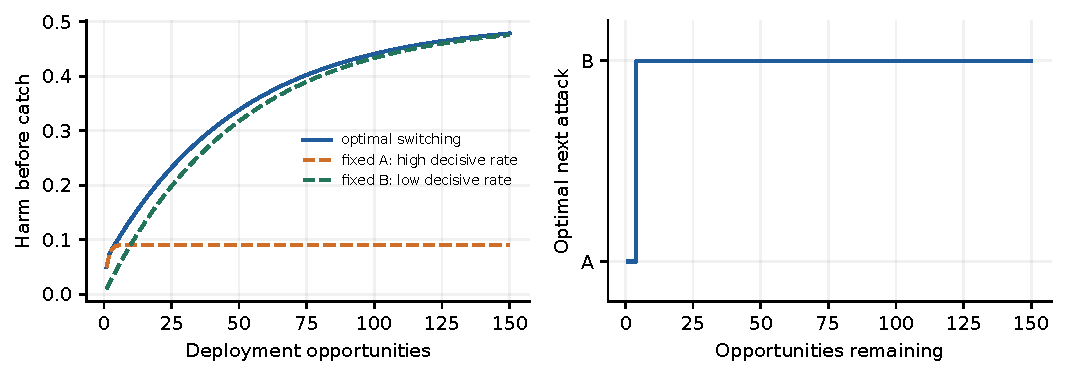
\includegraphics[width=\linewidth]{switching.pdf}
\caption{Controlled example. A has $(u,c)=(0.05,0.50)$ and B has $(0.01,0.01)$. Left: exact risks. Right: optimal next action versus opportunities remaining. All curves are model calculations.}\label{fig:switching}\end{figure}

\paragraph{Numerical implementation.}
The reference recursion uses $O(KT)$ time and $O(K)$ working memory for one interval. The optional accelerator applies Theorem~\ref{thm:switch} to the upper operator. It retains decisive probabilities directly and uses \texttt{log1p} and \texttt{expm1} for geometric updates, avoiding subtraction of a tiny decisive rate from one before a long-horizon calculation. The theory uses exact real arithmetic; the implementation uses double precision with independent numerical checks. It is not an interval-arithmetic proof certificate.

\subsection{Zero-harm and all-neutral evidence}
When $U_j=0$ and $M_j=m>0$, the exact conditional upper limit is
\begin{equation}r_j^+=1-\eta^{1/m}.\end{equation}
Since $R_T\leq r_j$, the sufficient all-horizon condition $r_j^+\leq\varepsilon$ requires
\begin{equation}m\geq\left\lceil\frac{\log\eta}{\log(1-\varepsilon)}\right\rceil.\label{eq:sample}\end{equation}
For a two-action 95\% joint envelope, $\eta=0.00625$; 5,073 decisive zero-harm observations per action suffice for a conditional harm-share bound of $0.001$. Neutral observations increase the evaluation sample size needed to obtain that decisive count. This is a sufficient condition for the construction, not an optimal sample-complexity claim.

\begin{proposition}[All-neutral evidence limit]\label{thm:neutral}
For one action and $n$ observations, any deterministic upper confidence bound for $R_T$ with coverage at least $1-\alpha$ uniformly over the three-outcome model must return at least $1-\alpha^{T/n}$ on the all-neutral count table.
\end{proposition}
\begin{proof}
Restrict to $c=0$, $u=p>0$. The all-neutral table has probability $(1-p)^n$ and true risk $1-(1-p)^T$. If its reported bound is below $1-\alpha^{T/n}$, choose $p<1-\alpha^{1/n}$ sufficiently close to that endpoint that true risk exceeds the reported bound. Noncoverage then occurs with probability greater than $\alpha$, contradicting the guarantee.
\end{proof}
At $T=n$, this necessary value is $1-\alpha$. Accurately resampling an all-neutral library cannot overcome this limit. The argument specializes a standard zero-event principle to deployment risk; the statistical phenomenon itself is not claimed as new.

\section{Computational study}\label{sec:study}
\subsection{Protocol and independent checks}
An internal prospective protocol was saved before the main run and is included as \texttt{PROTOCOL.txt}; it was not externally preregistered. The primary study uses six fixed menus (Table~\ref{tab:menus}), four fixed sample sizes $n\in\{50,200,1000,5000\}$ per action, horizon 100, and 10,000 independently generated datasets per condition. The seed is 1720406. Each dataset contains two independent multinomial count tables and is assessed by both separately calibrated methods with $\delta=0.05$. Primary endpoints are coverage, mean width, signed plug-in error, and zero plug-in frequency when true risk is positive. Monte Carlo standard errors use independent datasets as the unit.

\begin{table}[ht]\centering\small
\begin{tabular}{lccc}\toprule
Condition & A: $(u,c)$ & B: $(u,c)$ & True $V_{100}$\\\midrule
Balanced & $(.02,.08)$ & $(.01,.02)$ & .320324\\
Rare & $(.0002,.001)$ & $(.0001,.0001)$ & .018857\\
Zero harm & $(0,.01)$ & $(0,.1)$ & .000000\\
Switching & $(.05,.5)$ & $(.01,.01)$ & .441189\\
Low catch & $(.01,.0001)$ & $(.005,.0002)$ & .631333\\
Asymmetric & $(.001,.3)$ & $(.03,.05)$ & .374910\\\bottomrule
\end{tabular}
\caption{Prespecified synthetic kernels. These are categorical environments, not measured model behaviors.}\label{tab:menus}\end{table}

Independent implementation checks enumerate exact rational probabilities of every two-action sequence up to horizon nine, compare hazard extrema to separate linear programs, compare factor extrema to rectangle corners, and enumerate exact binomial tail errors. At $n=8$ per action, all $45^2=2,025$ joint count tables are enumerated at horizons 1, 5, and 20 for each menu, yielding 36 exact coverage calculations across both methods. A second enumeration uses all 5,151 one-action count tables at $n=100$ for the specified bootstrap baseline. No new model trajectory, API request, or training run is part of this study.

\subsection{Coverage and informativeness}
Across 24 primary conditions, factor coverage ranges from $0.9901$ to $1.0000$ and hazard-box coverage from $0.9964$ to $1.0000$. At the lowest factor coverage, Monte Carlo standard error is $0.00099$. These values show substantial conservatism rather than exact nominal calibration. Exact enumeration at $n=8$ gives minimum coverage $0.999628$ for factor envelopes and $0.994158$ for hazard boxes.

Figure~\ref{fig:width} and Table~\ref{tab:width} show why coverage alone is insufficient. Factor envelopes are narrower in several balanced or asymmetric cases, while hazard boxes are narrower for rare and low-catch cases at larger $n$. Neither uniformly dominates. Broad intervals can remain practically inconclusive despite correct coverage.

\begin{figure}[ht]\centering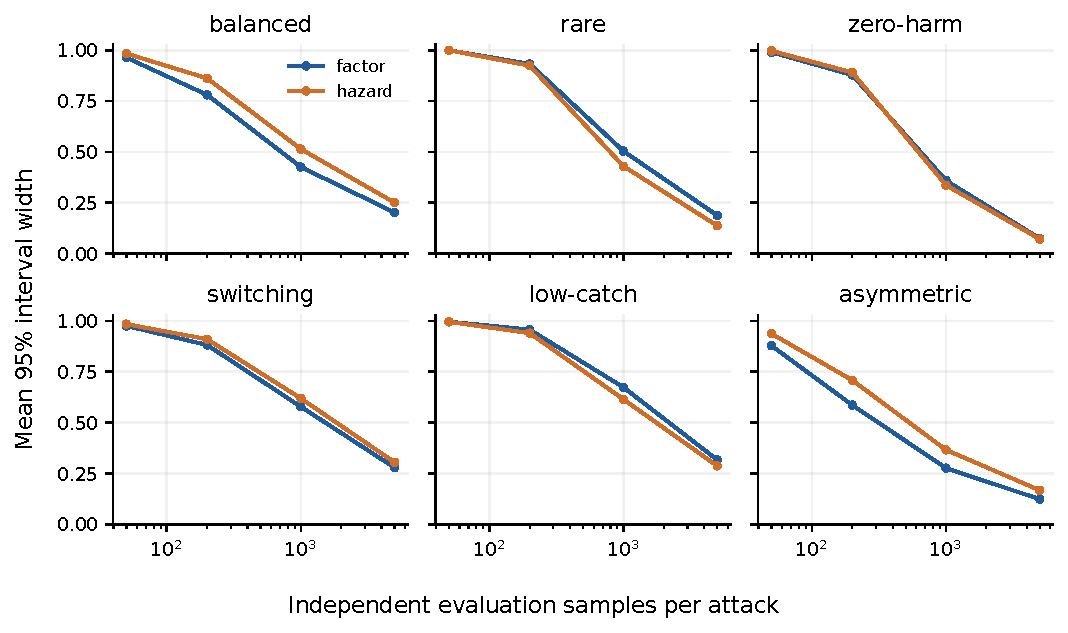
\includegraphics[width=\linewidth]{interval_widths.pdf}
\caption{Mean interval widths over 10,000 simulated datasets per point. Each method has a separate 95\% joint guarantee. Lines join tested sample sizes rather than a fitted scaling law.}\label{fig:width}\end{figure}

\begin{table}[ht]\centering\small
\begin{tabular}{lrrrr}\toprule
&\multicolumn{2}{c}{$n=1,000$}&\multicolumn{2}{c}{$n=5,000$}\\
Condition & Factor & Hazard & Factor & Hazard\\\midrule
Balanced & .4254 & .5138 & .2012 & .2501\\
Rare & .5036 & .4295 & .1872 & .1365\\
Zero harm & .3585 & .3359 & .0736 & .0706\\
Switching & .5779 & .6191 & .2783 & .3045\\
Low catch & .6735 & .6146 & .3169 & .2869\\
Asymmetric & .2762 & .3656 & .1231 & .1672\\\bottomrule
\end{tabular}
\caption{Mean interval widths. The largest Monte Carlo standard error among these entries is below $0.00068$. All conditions and errors are retained in the result CSV.}\label{tab:width}\end{table}

In the rare condition, $V_{100}=0.018857$, but the plug-in estimate is zero in 98.48\%, 93.97\%, 73.72\%, and 22.11\% of datasets at $n=50,200,1000,5000$. At $n=1000$, its mean is nevertheless $0.026331$: rare positive estimates and maximization across actions can reverse mean bias. Zero-estimate frequency and average error therefore describe different phenomena. In the zero-harm condition, every plug-in estimate is correctly zero, while confidence limits remain positive because they must also cover nearby harmful kernels.

\paragraph{Specified conditional bootstrap.}
The baseline conditions on $M=m$, bootstraps $m$ decisive labels at $\widehat r=U/m$, takes their exact 95th-percentile binomial share, and multiplies by $1-(1-m/n)^{100}$. For $m=0$ it returns zero. This deliberately holds decisive frequency fixed. In the first rare action, $(u,c)=(0.0002,0.001)$, exact upper coverage is $0.019803$, versus $1.000000$ for the factor bound. The zero-harm-observation probability is $0.980197$. The result establishes failure of this conditional procedure in this regime; it does not show that every bootstrap fails or that a maintained framework has this exact coverage.

\subsection{Exploratory accelerator verification}
The block accelerator was added after the primary study and logged separately. For $K\in\{2,8,32\}$, its upper values at horizons 100 and 10,000 agree with the reference recursion within $10^{-12}$. It also evaluates horizons $10^6$ and $10^{12}$. The generated confidence rectangles reach their limiting region quickly, so timings are illustrative rather than a worst-case benchmark. Separate tests compare 125 random menus with 1--16 actions to unrolled Bellman calculations and compare a $10^{-12}$ decisive probability at horizon $10^{12}$ to 60-digit decimal arithmetic. Computation speed is not a statistical-efficiency result.

\section{Secondary analysis of published aggregates}\label{sec:public}
The public factorial repository \citep{williams} describes a 24-cell planned attacker--monitor design. We pin commit \texttt{3e420c9a8180163eafaf35db17da0973d49fbd4a}. The checkout includes full-precision aggregate CSVs but no evaluation transcripts. We retain four monitor panels with both viable attacker rows and constant zero honest scores in both rows. The source's strict threshold above the maximum honest score is then the common threshold zero. Its documented sample size is 100 per mode per cell.

For published successful-attack count $A$, fraction $d$ of all attempts above threshold, and fraction $d_s$ of successful attempts above threshold, reconstruct
\begin{equation}C=100d,\qquad U=A(1-d_s),\qquad N=100-U-C.\end{equation}
Every count must be within $10^{-8}$ of an integer. Catch includes unsuccessful attempts above threshold, following the source convention. Such events would only justify the absorbing catch model if an audit establishes subversion and stops the deployment before harm.

\begin{table}[ht]\centering\small
\begin{tabular}{lrrr|rrr}\toprule
&\multicolumn{3}{c}{Gemini attacker}&\multicolumn{3}{c}{GPT attacker}\\
Monitor &$U$&$C$&$N$&$U$&$C$&$N$\\\midrule
Gemini 3.1 Pro &41&33&26&11&39&50\\
GPT-4.1 mini &60&13&27&24&21&55\\
GPT-5.5 &34&43&23&9&41&50\\
Opus 4.8 &34&49&17&9&43&48\\\bottomrule
\end{tabular}
\caption{Aggregate-derived counts, not new model experiments. Each panel has two 100-attempt cells. Names follow the upstream registry; unavailable transcripts prevent independent verification of outcomes and model identities.}\label{tab:counts}\end{table}

\paragraph{Selection amendment.}
The source excluded attacker rows using observed success counts. Our prospective plan initially corrected over eight retained cells. On identifying this outcome-dependent selection, we expanded the correction to all 24 planned cells, after viewing initial results and before writing the manuscript. This amendment appears in \texttt{DEVIATIONS.txt}. A union bound over the original family permits subsequent subset reporting under the sampling assumptions; it does not repair selective completion, non-IID sampling, or missing logs.

Figure~\ref{fig:public} uses $\eta=0.05/(4\cdot24)$. For the four panels, plug-in risks and intervals at horizon 100 are respectively $0.5541\,[0.3602,0.7369]$, $0.8219\,[0.6394,0.9379]$, $0.4416\,[0.2626,0.6319]$, and $0.4096\,[0.2413,0.5943]$. These intervals do not establish a strict ranking of all four candidates. The first attacker maximizes risk at every tested horizon in each panel; switching adds no observed plug-in gain here. The switching effect is established by the controlled example, not these aggregates.

\begin{figure}[ht]\centering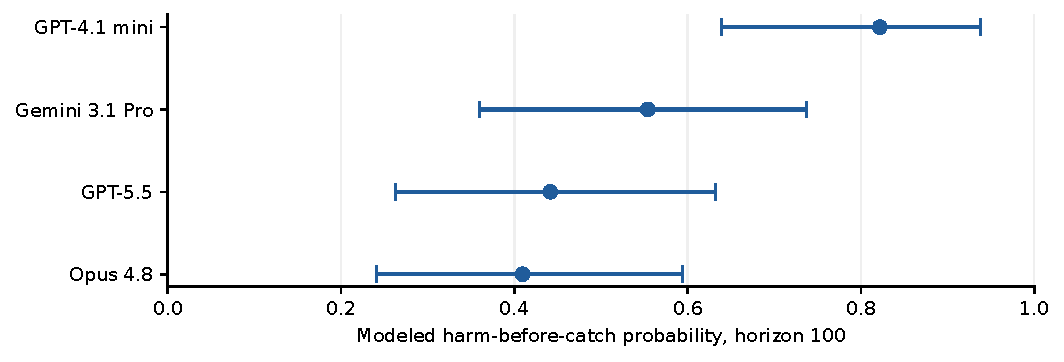
\includegraphics[width=\linewidth]{public_intervals.pdf}
\caption{Model-conditional intervals for optimal risk within the two reported attacker kernels, horizon 100. The correction covers the original 24-cell design. Strong-model monitors are diagnostic comparisons, not claims of trustworthiness.}\label{fig:public}\end{figure}

\paragraph{Interpretation limits.}
Shared generations across monitors create cross-cell dependence, which the union bound permits. The within-cell IID interpretation remains unverified: a fixed benchmark task list need not be a random sample of deployment. Source labels are accepted rather than reproduced. Zero empirical false alarms does not prove zero future false alarms, and resource feasibility is untested. These are model-conditional calculations from reported aggregates, not independently validated deployment certificates or a replication of model performance.

\section{Practical implications and limitations}
A plausible commercial application is an evidence-reporting component for agent evaluation: given validated categorical logs, it associates a risk statement with its attack menu, horizon, uncertainty allocation, and shutdown assumptions. It can identify where more evidence is needed before a specified deployment review. This is a proposed use, not measured market demand, a revenue forecast, or a claim of patentability.

The main practical lesson is that correct coverage can coexist with poor precision. A declared-family decision at tolerance $\varepsilon$ may require $W_T\leq\varepsilon$. Failing this condition means that present evidence does not support that assertion; it does not prove the system violates the tolerance. The zero-harm and rare-event experiments make this distinction concrete.

The menu is finite and fixed. Untested attacks are excluded. Sample sizes are fixed rather than adaptively stopped. Deployment choices precede new outcomes and do not reveal context that changes the kernel. Detection is immediate and effective, labels are correct, and deployment kernels match evaluation. Audit-budget exhaustion, delayed review, and audit-stage false negatives can invalidate the model. None of these assumptions follows from the confidence theorem.

The construction is conservative because of marginal error allocation, confidence rectangles, and per-step parameter reselection. A joint multinomial likelihood region with fixed-kernel optimization could tighten the result. Resource-dependent deployments need more states; anytime evaluation needs confidence sequences. A substantive next empirical study should independently sample tasks under a frozen attack menu, calibrate a common monitor on a separate split, verify catch-to-shutdown timing, and compare held-out deployment outcomes to the envelopes. That study has not been conducted here.

\section{Conclusion}
StopRisk maps finite categorical evidence to harm-before-shutdown envelopes for a declared menu of stationary attacks. Conditional binomial inference and robust Bellman propagation give simultaneous coverage across horizons and adaptive within-menu selection. The optimistic operator admits bounded-switch block evaluation. Exact checks and controlled simulations support implementation correctness while revealing substantial uncertainty and no universal width advantage. The artifact provides a precise account of what a specified evaluation supports, conditional on its deployment model and tested attack boundary.

\paragraph{Availability.}
Source, protocol, amendments, attributed public aggregates, synthetic count tables, results, figures, and manuscript source are available at \url{https://github.com/shi1720/stoprisk}. Reproduction needs no model credentials. The package does not contain raw model transcripts.

\begin{thebibliography}{20}
\bibitem[Greenblatt et~al.(2024)]{greenblatt} Ryan Greenblatt, Buck Shlegeris, Fabien Roger, and Nate Sachan. AI Control: Improving Safety Despite Intentional Subversion. \emph{ICML}, 2024. \url{https://arxiv.org/abs/2312.06942}.
\bibitem[Griffin et~al.(2024)]{griffin} Charlie Griffin, Louis Thomson, Buck Shlegeris, and Alessandro Abate. Games for AI Control: Models of Safety Evaluations of AI Deployment Protocols. arXiv:2409.07985, 2024. \url{https://arxiv.org/abs/2409.07985}.
\bibitem[Ge-Wang et~al.(2026)]{gewang} Catherine Ge-Wang, Tyler Crosse, Benjamin Hadad IV, Joachim Schaeffer, Ram Potham, and Tyler Tracy. Attack Selection in Agentic AI Control Evaluations Meaningfully Decreases Safety. arXiv:2606.06529, 2026. \url{https://arxiv.org/abs/2606.06529}.
\bibitem[Clopper and Pearson(1934)]{clopper} C.~J. Clopper and E.~S. Pearson. The Use of Confidence or Fiducial Limits Illustrated in the Case of the Binomial. \emph{Biometrika}, 26(4):404--413, 1934. \url{https://doi.org/10.1093/biomet/26.4.404}.
\bibitem[Iyengar(2005)]{iyengar} Garud~N. Iyengar. Robust Dynamic Programming. \emph{Mathematics of Operations Research}, 30(2):257--280, 2005. \url{https://doi.org/10.1287/moor.1040.0129}.
\bibitem[Nilim and El Ghaoui(2005)]{nilim} Arnab Nilim and Laurent El Ghaoui. Robust Control of Markov Decision Processes with Uncertain Transition Matrices. \emph{Operations Research}, 53(5):780--798, 2005. \url{https://people.eecs.berkeley.edu/~elghaoui/Pubs/RobMDP_OR2005.pdf}.
\bibitem[Blanche(2020)]{blanche} Paul Blanche. Confidence intervals for the cumulative incidence function via constrained NPMLE. \emph{Lifetime Data Analysis}, 26:45--64, 2020. \url{https://doi.org/10.1007/s10985-018-09458-6}.
\bibitem[Varonka and Watanabe(2025)]{varonka} Anton Varonka and Kazuki Watanabe. On Piecewise Affine Reachability with Bellman Operators. \emph{MFCS 2025}, LIPIcs 345, 92:1--92:18. \url{https://doi.org/10.4230/LIPIcs.MFCS.2025.92}.
\bibitem[ControlArena contributors(2026)]{controlarena} ControlArena contributors. ControlArena: Analysis utilities and tutorial. Software, commit \texttt{20857c9de7f5e892ab8d9ec8b5fb510a1768b977}; accessed 17 October 2026. \url{https://control-arena.aisi.org.uk/analysis.html}; \url{https://github.com/UKGovernmentBEIS/control-arena}.
\bibitem[Williams(2026)]{williams} Andre Williams. Trusted Monitoring: Monitor Identity Beats Monitor Tier. Public repository, commit \texttt{3e420c9a8180163eafaf35db17da0973d49fbd4a}; accessed 17 October 2026. \url{https://github.com/Andre-Williams22/trusted-monitoring-factorial-research}.
\bibitem[TMLS AI Research(2026)]{tmls} TMLS AI Research. The Red-Team / Blue-Team Game: Equilibria, Convergence, and a Stopping Rule for AI Assurance. Online research essay, 16 July 2026. \url{https://www.tmls.nyc/research/game-theoretic-redteam}.
\end{thebibliography}

\appendix
\section{Minimal executable example}
The following calculation reproduces the analytical switching value. The count inputs are illustrative, not presented as observations from model calls.
\begin{lstlisting}[language=Python]
from stoprisk import Counts, confidence_rectangles, envelope, optimal_risk
from stoprisk.fast import factor_upper_fast

v = optimal_risk([.05, .01], [.50, .01], horizon=10)
assert abs(float(v) - .13766610556115022) < 1e-12

data = [Counts(n=1000, harm=50, caught=500),
        Counts(n=1000, harm=10, caught=10)]
rect = confidence_rectangles(data, delta=.05)
lo, hi = envelope(rect, horizon=100)
fast_hi, blocks = factor_upper_fast(rect, horizon=100)
assert abs(float(hi) - fast_hi) < 1e-12
print(float(lo), float(hi), blocks)
\end{lstlisting}
To reproduce the numerical study in a new environment, use:
\begin{lstlisting}
python -m pip install -e '.[research]'
python -m pytest -q
python scripts/run_study.py
python scripts/make_figures.py
tectonic manuscript/main.tex
\end{lstlisting}
The lock file records the executed package versions. Reference and accelerated operators are separate implementations. Tests use exact rational probabilities, separate numerical linear programs, exhaustive count-table probabilities, and high-precision decimal arithmetic as independent oracles.

\section{Perturbation with absorption}
Kernel uncertainty need not be multiplied by a long horizon without regard to absorption. Suppose two menu operators $F,G$ have decisive probabilities at least $s_0>0$ for all component maps and $\sup_{v\in[0,1]}|F(v)-G(v)|\leq e$. Both are Lipschitz with constant at most $1-s_0$. Induction gives
\begin{equation}
|F^T(0)-G^T(0)|\leq e\sum_{i=0}^{T-1}(1-s_0)^i
=e\frac{1-(1-s_0)^T}{s_0}.
\end{equation}
This is the usual absorbing/discounted dynamic-programming perturbation argument specialized to the scalar model. If the confidence set permits $s_0=0$, this argument yields only $Te$. Rare decisive events therefore matter both for inference and uncertainty propagation. No optimal rate for the proposed confidence rectangles follows from this observation.

\section{Artifact and amendment record}
The artifact separates upstream aggregates, derived counts, synthetic counts, and results. The prospective protocol and post-run amendments are retained in \texttt{PROTOCOL.txt} and \texttt{DEVIATIONS.txt}. Runtime versions and main-run hashes appear in \texttt{results/run\_manifest.json}; \texttt{SHA256SUMS.txt} covers final package files.
\end{document}
